\documentclass[aspectratio=169,11pt]{beamer}

\usetheme{Madrid}
\usecolortheme{dolphin}
\setbeamertemplate{navigation symbols}{}
\setbeamertemplate{footline}[frame number]

\usepackage{amsmath,amssymb,booktabs,array}
\usepackage{tikz}
\usetikzlibrary{arrows.meta,positioning,shapes.geometric,calc}

\definecolor{polyunavy}{RGB}{20,58,90}
\definecolor{polyublue}{RGB}{48,96,135}
\definecolor{polyuaccent}{RGB}{168,74,62}
\definecolor{polyugreen}{RGB}{43,118,89}
\definecolor{softblue}{RGB}{231,241,248}
\definecolor{softgreen}{RGB}{232,244,239}
\definecolor{softred}{RGB}{252,238,236}
\definecolor{ink}{RGB}{34,40,46}

\setbeamercolor{title}{fg=white,bg=polyunavy}
\setbeamercolor{frametitle}{fg=white,bg=polyunavy}
\setbeamercolor{structure}{fg=polyublue}
\setbeamercolor{block title}{fg=white,bg=polyublue}
\setbeamercolor{block body}{fg=ink,bg=softblue}
\setbeamercolor{alertblock title}{fg=white,bg=polyuaccent}
\setbeamercolor{alertblock body}{fg=ink,bg=softred}
\setbeamercolor{exampleblock title}{fg=white,bg=polyugreen}
\setbeamercolor{exampleblock body}{fg=ink,bg=softgreen}

\title[Robust Crew Pairing]{Incremental Data-Driven Robust Crew Pairing Optimization}
\subtitle{Under Evolving Delay Uncertainty}
\author[Xinyu HUANG]{Xinyu HUANG}
\institute[PolyU]{Department of Industrial and Systems Engineering\\The Hong Kong Polytechnic University}
\date{}

\newcommand{\smallcite}[1]{\textcolor{polyublue}{\scriptsize #1}}
\newcommand{\stagebox}[2]{%
  \begin{block}{#1}
  #2
  \end{block}
}
\newenvironment{compactitem}{%
  \begin{itemize}
  \setlength{\itemsep}{1pt}
  \setlength{\parskip}{0pt}
}{\end{itemize}}

\begin{document}

% Assessment 2 alignment:
% - Approximately 12 minutes plus Q&A.
% - Communicate specialized research to a non-specialist audience.
% - Must include Methods and Procedures, Results and Discussion, and Conclusion.
% - Avoid reading a script; use slides as visual support and signposting.

\begin{frame}{Introduction: delays turn cheap crew schedules into costly ones}
  \begin{center}
  \resizebox{0.95\textwidth}{!}{%
  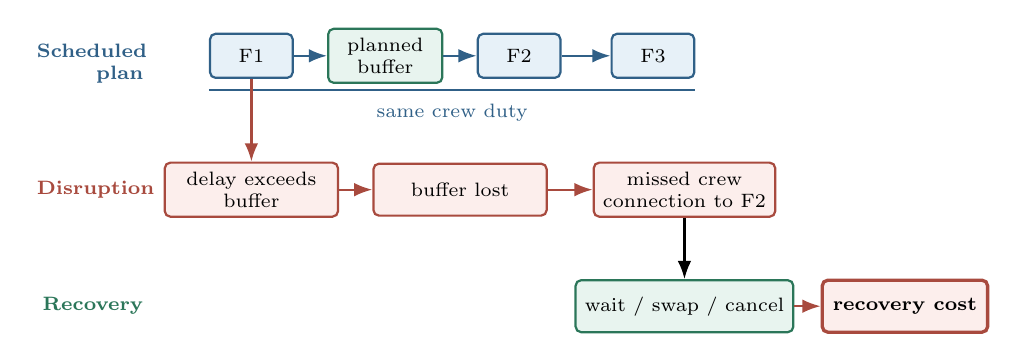
\begin{tikzpicture}[
    flight/.style={draw=polyublue,thick,rounded corners=2pt,fill=softblue,
      minimum width=1.05cm,minimum height=0.56cm,align=center,font=\scriptsize},
    buffer/.style={draw=polyugreen,thick,rounded corners=2pt,fill=softgreen,
      minimum width=1.45cm,minimum height=0.56cm,align=center,font=\scriptsize},
    risk/.style={draw=polyuaccent,thick,rounded corners=2pt,fill=softred,
      minimum width=2.20cm,minimum height=0.66cm,align=center,font=\scriptsize},
    action/.style={draw=polyugreen,thick,rounded corners=2pt,fill=softgreen,
      minimum width=2.35cm,minimum height=0.66cm,align=center,font=\scriptsize},
    cost/.style={draw=polyuaccent,very thick,rounded corners=2pt,fill=softred,
      minimum width=2.10cm,minimum height=0.66cm,align=center,font=\scriptsize\bfseries},
    lane/.style={font=\scriptsize\bfseries,align=right,text=polyublue,text width=1.35cm},
    arr/.style={-Latex,thick}
  ]
    \node[lane,anchor=east] at (-5.10,1.60) {Scheduled\\plan};
    \node[flight] (f1) at (-3.85,1.70) {F1};
    \node[buffer] (buf) at (-2.15,1.70) {planned\\buffer};
    \node[flight] (f2) at (-0.45,1.70) {F2};
    \node[flight] (f3) at (1.25,1.70) {F3};

    \draw[arr,draw=polyublue] (f1) -- (buf);
    \draw[arr,draw=polyublue] (buf) -- (f2);
    \draw[arr,draw=polyublue] (f2) -- (f3);
    \draw[thick,draw=polyublue]
      ($(f1.south west)+(0,-0.14)$) -- ($(f3.south east)+(0,-0.14)$);
    \node[font=\scriptsize,text=polyublue] at (-1.30,0.98) {same crew duty};

    \node[lane,text=polyuaccent,anchor=east] at (-5.10,0.00) {Disruption};
    \node[risk] (delay) at (-3.85,0.00) {delay exceeds\\buffer};
    \node[risk] (lost) at (-1.20,0.00) {buffer lost};
    \node[risk] (miss) at (1.65,0.00) {missed crew\\connection to F2};

    \draw[arr,draw=polyuaccent] (f1.south) -- (delay.north);
    \draw[arr,draw=polyuaccent] (delay) -- (lost);
    \draw[arr,draw=polyuaccent] (lost) -- (miss);

    \node[lane,text=polyugreen,anchor=east] at (-5.10,-1.48) {Recovery};
    \node[action] (recover) at (1.65,-1.48) {wait / swap / cancel};
    \node[cost] (rcost) at (4.45,-1.48) {recovery cost};
    \draw[arr] (miss) -- (recover);
    \draw[arr,draw=polyuaccent] (recover) -- (rcost);
  \end{tikzpicture}
  }
  \end{center}

  \vspace{0.08cm}
  \begin{center}
    \small\textbf{\textcolor{polyuaccent}{Motivation:}}
    A schedule that is cheap on paper may become expensive when a delay breaks crew connections.
  \end{center}
\end{frame}

\begin{frame}
  \titlepage
  \vspace{-0.35cm}
  \begin{center}
    \small Research question: How can airline crew schedules stay reliable when delay patterns keep changing?
  \end{center}
\end{frame}

\begin{frame}{Introduction: this motivates the research question}
  \begin{columns}[T,onlytextwidth]
    \column{0.50\textwidth}
      \textbf{Key terms}
      \begin{itemize}
        \item \textbf{Crew pairing:} a sequence of flights assigned to one crew duty plan.
        \item \textbf{Delay propagation:} one delayed flight breaks a later crew connection.
        \item \textbf{Robust schedule:} a plan designed to remain workable under severe but plausible delays.
      \end{itemize}

      \begin{alertblock}{Why this matters}
        Planning should consider recovery cost, not only planned operating cost.
      \end{alertblock}

    \column{0.45\textwidth}
      \begin{exampleblock}{Research question}
        How can we design crew pairings that balance planned operating cost and recovery cost when delay patterns keep changing?
      \end{exampleblock}

      \textbf{Presentation roadmap}
      \begin{itemize}
        \item Literature review: what tools already exist?
        \item Methods: how is the model built and solved?
        \item Results and discussion: what can be concluded now?
      \end{itemize}
  \end{columns}
\end{frame}

\begin{frame}{Literature review: useful tools are available, but not combined}
  \begin{columns}[T,onlytextwidth]
    \column{0.48\textwidth}
      \begin{block}{Crew pairing models}
        Build schedules that satisfy duty, rest, and connection rules.
      \end{block}
      \begin{block}{Robust optimization}
        Control conservatism with an uncertainty budget. \smallcite{Bertsimas and Sim, 2004}
      \end{block}

    \column{0.48\textwidth}
      \begin{block}{Two-stage robust optimization}
        Separate pre-delay planning from post-delay recovery. \smallcite{Zeng and Zhao, 2013}
      \end{block}
      \begin{block}{Delay-robust transport models}
        Use one-sided bounds for late-arrival uncertainty. \smallcite{Wang and Qi, 2020}
      \end{block}
  \end{columns}

  \vspace{0.12cm}
  \begin{alertblock}{Research gap}
    Gap: no unified framework combining data-driven delay bounds, recovery decisions, and incremental re-optimization for robust crew pairing.
  \end{alertblock}
\end{frame}

\begin{frame}{Methods and procedures: the proposed framework has four stages}
  \begin{center}
  \resizebox{0.95\textwidth}{!}{%
  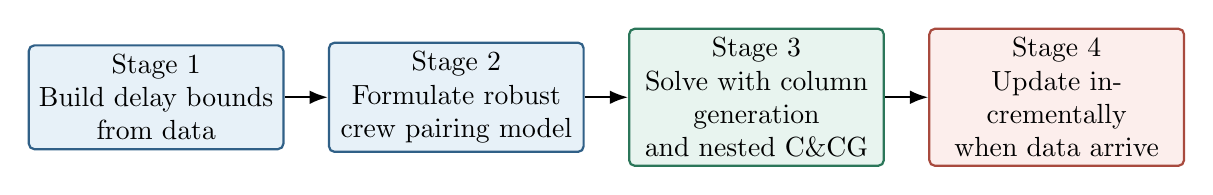
\begin{tikzpicture}[
    stage/.style={draw=polyublue,thick,rounded corners=2pt,fill=softblue,
      align=center,text width=3.0cm,minimum height=1.0cm},
    green/.style={draw=polyugreen,thick,rounded corners=2pt,fill=softgreen,
      align=center,text width=3.0cm,minimum height=1.0cm},
    red/.style={draw=polyuaccent,thick,rounded corners=2pt,fill=softred,
      align=center,text width=3.0cm,minimum height=1.0cm},
    arr/.style={-Latex,thick}
  ]
    \node[stage] (s1) {Stage 1\\Build delay bounds\\from data};
    \node[stage,right=0.55cm of s1] (s2) {Stage 2\\Formulate robust\\crew pairing model};
    \node[green,right=0.55cm of s2] (s3) {Stage 3\\Solve with column generation\\and nested C\&CG};
    \node[red,right=0.55cm of s3] (s4) {Stage 4\\Update incrementally\\when data arrive};
    \draw[arr] (s1) -- (s2);
    \draw[arr] (s2) -- (s3);
    \draw[arr] (s3) -- (s4);
  \end{tikzpicture}
  }
  \end{center}

  \vspace{0.25cm}
  \begin{exampleblock}{The key idea}
    The framework searches for crew schedules that are affordable in advance and easier to recover after severe delays.
  \end{exampleblock}
\end{frame}

\begin{frame}{Stage 1: delay data become delay bounds}
  \begin{columns}[T,onlytextwidth]
    \column{0.48\textwidth}
      \textbf{Input to output}

      Historical delay data are converted into one-sided delay bounds.

      \vspace{0.20cm}
      \begin{block}{Numerical example}
        \begin{center}
        \small
        Historical delays (min)\\[0.05cm]
        \[
        \begin{array}{rrrrr}
        5 & 8 & 12 & 13 & 18\\
        20 & 25 & 31 & 40 & 52
        \end{array}
        \]
        90\% quantile\\[-0.02cm]
        \(\downarrow\)\\[-0.02cm]
        \textbf{Delay bound = 40 min}
        \end{center}
      \end{block}

    \column{0.48\textwidth}
      \textbf{Formula}
      \[
        d_f=\operatorname{Quantile}_{\alpha}
        (x_f^1,x_f^2,\ldots,x_f^T)
      \]
      \[
        0\leq \Delta_f \leq d_f
      \]

      \begin{alertblock}{Interpretation}
        The model prepares for severe but realistic late arrivals.
      \end{alertblock}
  \end{columns}
\end{frame}

\begin{frame}{Stage 2: the model balances planned operating cost and recovery cost}
  \begin{center}
  \begin{block}{Core optimization objective}
    \[
      \min_x\{\text{planned operating cost}
      +\text{worst-case recovery cost}\}
    \]
  \end{block}
  \end{center}

  \begin{exampleblock}{Trade-off}
    A slightly higher planned operating cost may reduce worst-case recovery cost.
  \end{exampleblock}

  \begin{alertblock}{Solved iteratively}
    The algorithm adds only useful pairings and difficult delay scenarios.
  \end{alertblock}
\end{frame}

\begin{frame}{Stage 3: the solution adds only useful pieces}
  \begin{center}
  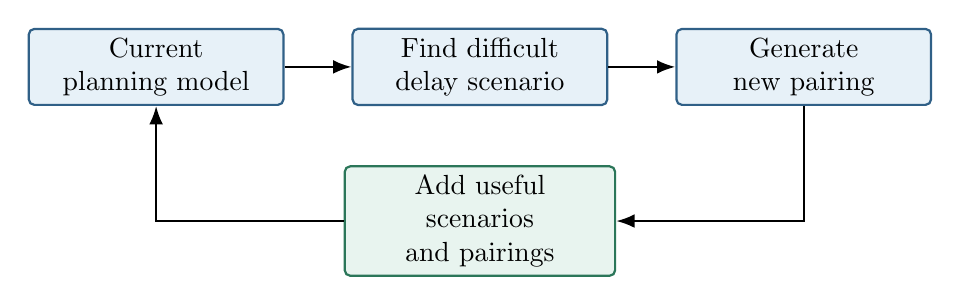
\begin{tikzpicture}[
    box/.style={draw=polyublue,thick,rounded corners=2pt,align=center,
      text width=3.0cm,minimum height=0.9cm,fill=softblue},
    green/.style={draw=polyugreen,thick,rounded corners=2pt,align=center,
      text width=3.2cm,minimum height=0.9cm,fill=softgreen},
    arr/.style={-Latex,thick}
  ]
    \node[box] (rmp) {Current\\planning model};
    \node[box,right=0.85cm of rmp] (sep) {Find difficult\\delay scenario};
    \node[box,right=0.85cm of sep] (price) {Generate\\new pairing};
    \node[green,below=0.75cm of sep] (add) {Add useful\\scenarios and pairings};
    \draw[arr] (rmp) -- (sep);
    \draw[arr] (sep) -- (price);
    \draw[arr] (price.south) |- (add.east);
    \draw[arr] (add.west) -| (rmp.south);
  \end{tikzpicture}
  \end{center}

  \begin{columns}[T,onlytextwidth]
    \column{0.48\textwidth}
      \begin{block}{Column generation}
        Generate a new crew pairing only when it can improve the plan.
      \end{block}
    \column{0.48\textwidth}
      \begin{block}{Nested C\&CG}
        Generate a difficult delay scenario only when the current plan fails under it.
      \end{block}
  \end{columns}
\end{frame}

\begin{frame}{Stage 4: new data trigger an incremental update}
  \begin{center}
  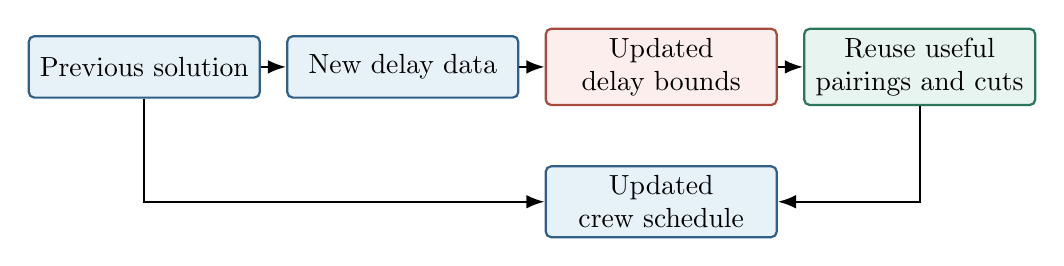
\begin{tikzpicture}[
    node distance=0.32cm,
    box/.style={draw=polyublue,thick,rounded corners=2pt,fill=softblue,
      align=center,text width=2.7cm,minimum height=0.78cm},
    red/.style={draw=polyuaccent,thick,rounded corners=2pt,fill=softred,
      align=center,text width=2.7cm,minimum height=0.78cm},
    green/.style={draw=polyugreen,thick,rounded corners=2pt,fill=softgreen,
      align=center,text width=2.7cm,minimum height=0.78cm},
    arr/.style={-Latex,thick}
  ]
    \node[box] (old) {Previous solution};
    \node[box,right=of old] (data) {New delay data};
    \node[red,right=of data] (bounds) {Updated delay bounds};
    \node[green,right=of bounds] (reuse) {Reuse useful pairings and cuts};
    \node[box,below=0.75cm of bounds] (new) {Updated crew schedule};
    \draw[arr] (old) -- (data);
    \draw[arr] (data) -- (bounds);
    \draw[arr] (bounds) -- (reuse);
    \draw[arr] (reuse.south) |- (new.east);
    \draw[arr] (old.south) |- (new.west);
  \end{tikzpicture}
  \end{center}

  \begin{columns}[T,onlytextwidth]
    \column{0.48\textwidth}
      \begin{block}{Technical term}
        An incremental update reuses the previous solution after new data arrive.
      \end{block}
    \column{0.48\textwidth}
      \begin{alertblock}{Why this matters}
        Fast updates matter because delay patterns change over time.
      \end{alertblock}
  \end{columns}
\end{frame}

\begin{frame}{Results and discussion: preliminary findings support the approach}
  \begin{columns}[T,onlytextwidth]
    \column{0.50\textwidth}
      \begin{exampleblock}{Finding 1}
        Search becomes more targeted as useful pairings and scenarios are added.
      \end{exampleblock}

      \begin{exampleblock}{Finding 2}
        Existing pairings and cuts can be reused after delay updates.
      \end{exampleblock}

    \column{0.45\textwidth}
      \begin{exampleblock}{Finding 3}
        Higher planned cost may reduce worst-case recovery cost.
      \end{exampleblock}

      \begin{alertblock}{Current status}
        \begin{compactitem}
          \item Preliminary analytical findings
          \item Numerical experiments ongoing
        \end{compactitem}
      \end{alertblock}
  \end{columns}
\end{frame}

\begin{frame}{Expected computational evaluation}
  \begin{columns}[T,onlytextwidth]
    \column{0.32\textwidth}
      \begin{block}{Nominal model}
        Low planned cost, but no explicit delay protection.
      \end{block}

    \column{0.32\textwidth}
      \begin{block}{Static robust model}
        Solves once with a fixed uncertainty set for delay protection.
      \end{block}

    \column{0.32\textwidth}
      \begin{block}{Incremental robust model}
        Updates after new delay data while reusing previous work.
      \end{block}
  \end{columns}

  \vspace{0.25cm}
  \begin{exampleblock}{Metrics}
    \begin{compactitem}
      \item Planned operating cost
      \item Worst-case recovery cost
      \item Total cost
      \item Runtime
    \end{compactitem}
  \end{exampleblock}

  \begin{alertblock}{Interpretation}
    Test whether incremental re-optimization saves time while maintaining recovery performance.
  \end{alertblock}
\end{frame}

\begin{frame}{Discussion: the comparison should reveal cost, reliability, and speed}
  \begin{columns}[T,onlytextwidth]
    \column{0.50\textwidth}
      \textbf{Expected pattern}
      \begin{compactitem}
        \item Nominal plans may look cheapest before delays.
        \item Static robustness should reduce recovery cost.
        \item Incremental robustness should update faster.
      \end{compactitem}

    \column{0.45\textwidth}
      \begin{alertblock}{Important qualification}
        Expected outcomes; experiments still needed.
      \end{alertblock}

      \begin{block}{Why this matters}
        The goal is a schedule that is affordable, reliable, and quick to update.
      \end{block}
  \end{columns}
\end{frame}

\begin{frame}{Conclusion: delay data can guide robust crew schedules}
  \begin{columns}[T,onlytextwidth]
    \column{0.48\textwidth}
      \textbf{Problem and method}
      \begin{compactitem}
        \item Delay propagation creates recovery cost.
        \item One-sided delay bounds represent late arrivals.
        \item Robust crew pairing balances planned and recovery cost.
      \end{compactitem}

    \column{0.48\textwidth}
      \textbf{Contribution and next step}
      \begin{compactitem}
        \item Incremental updates reuse previous work.
        \item Faster re-optimization supports changing data.
        \item Numerical experiments will test the benefit.
      \end{compactitem}

      \begin{alertblock}{Takeaway}
        Reliable schedules without excessive re-optimization time.
      \end{alertblock}
  \end{columns}
\end{frame}

\begin{frame}{Q\&A}
  \begin{center}
    \vspace{0.7cm}
    {\Large Thank you}\\[0.35cm]
    {\large Questions are welcome}\\[0.55cm]

    \begin{block}{Possible discussion points}
      Delay data, recovery actions, model comparison, or future numerical experiments.
    \end{block}
  \end{center}
\end{frame}

\end{document}
